\documentclass[12pt, a4paper]{report} % Classe report per tesi e relazioni, 12pt per una dimensione del testo più leggibile, a4paper per il formato carta europeo

% --- PACCHETTI ---
\usepackage[utf8]{inputenc}  % Per la codifica UTF-8
\usepackage[T1]{fontenc}     % Per una migliore gestione dei font
\usepackage[italian]{babel}  % Per la lingua italiana
\usepackage{graphicx}        % Per le immagini
\usepackage{xcolor}          % Per i colori
\usepackage{geometry}        % Per i margini
\usepackage{titlesec}        % Per i titoli
\usepackage{float}           % Per il posizionamento delle figure
\usepackage{fancyhdr}        % Per intestazioni e piè di pagina personalizzati
\usepackage{listings}        % Per il codice
\usepackage{tabularx}        % Per tabelle che si adattano alla larghezza
\usepackage{times}           % Font stile Times come nel template di riferimento
\usepackage{hyperref}        % Per i link ipertestuali

% --- CONFIGURAZIONE LINK E COLORI ---
\definecolor{linkblue}{RGB}{0, 0, 238}
\definecolor{darkblue}{RGB}{0, 0, 139}

\hypersetup{
    colorlinks=true,
    linkcolor=linkblue,
    filecolor=magenta,
    urlcolor=blue,
    pdftitle={EscapeManager - Relazione Progetto},
    pdfauthor={Adriano Luca Castaldo},
}

% --- CONFIGURAZIONE MARGINI ---
\geometry{
    left=25mm,
    right=25mm,
    top=25mm,
    bottom=25mm,
    headheight=15pt
}

% --- CONFIGURAZIONE HEADER E FOOTER (Fancyhdr) ---
\pagestyle{fancy}
\fancyhf{}
 
% Header
\fancyhead[L]{\textit{Adriano Luca Castaldo}}
\fancyhead[R]{\textit{Ingegneria del Software}}
 
% Footer
\fancyfoot[C]{\thepage}

\fancypagestyle{plain}{
  \fancyhf{}
  \fancyfoot[C]{\thepage}
  \renewcommand{\headrulewidth}{0pt}
}

% --- CONFIGURAZIONE CODICE JAVA ---
\definecolor{javared}{rgb}{0.6,0,0}
\definecolor{javagreen}{rgb}{0.25,0.5,0.35}
\definecolor{javapurple}{rgb}{0.5,0,0.35}
\definecolor{javadocblue}{rgb}{0.25,0.35,0.75}

\lstset{
    language=Java,
    basicstyle=\ttfamily\small,
    keywordstyle=\color{javapurple}\bfseries,
    stringstyle=\color{javared},
    commentstyle=\color{javagreen},
    morecomment=[s][\color{javadocblue}]{/**}{*/},
    numbers=left,
    numberstyle=\tiny\color{gray},
    stepnumber=1,
    numbersep=10pt,
    tabsize=4,
    showspaces=false,
    showstringspaces=false,
    frame=single,
    rulecolor=\color{black!30},
    breaklines=true,
    captionpos=b
}

\title{Applicativo Java EscapeManager}
\author{Adriano Luca Castaldo}

% --- TEMPLATE TESTI FRONTESPIZIO ---
\newcommand{\CoverUniversity}{Università degli Studi di Firenze}
\newcommand{\CoverDepartment}{Dipartimento di Ingegneria dell'Informazione}
\newcommand{\CoverCourse}{Ingegneria del software}
\newcommand{\CoverProfessor}{Enrico Vicario}
\newcommand{\CoverStudentId}{7138545}

\begin{document}

% --- FRONTESPIZIO ---
\begin{titlepage}
    \newcommand{\HRule}{\rule{\linewidth}{0.5mm}}

  \centering
    
\includegraphics[width=14cm]{images/logo_unifi.png}\\[1cm]

  \textsc{\LARGE \CoverUniversity}\\[0.5cm]
  \textsc{\Large \CoverDepartment}\\[0.5cm]

    \makeatletter
    \HRule \\[1cm]
    { \huge \bfseries \@title}\\[0.7cm]
    \HRule \\[1.2cm]

    \begin{minipage}{0.4\textwidth}
      \begin{flushleft} \large
        \textit{Autore:}\\
        \@author
        \\[1.2em]
        \textit{N$^{\circ}$ Matricola:}\\
        \CoverStudentId \\[1.2em]
      \end{flushleft}
    \end{minipage}
    ~
    \begin{minipage}{0.4\textwidth}
      \begin{flushright} \large
        \textit{Corso principale:} \\
        \CoverCourse\\[1.2em]
        \textit{Docente corso:} \\
        \CoverProfessor
      \end{flushright}
    \end{minipage}\\[2cm]
    \makeatother

    \vfill

    \centering
    {\large Anno Accademico 2025/2026}
\end{titlepage}

% --- INDICE ---
{
  \hypersetup{linkcolor=blue}
  \tableofcontents
}
\newpage

% --- CAPITOLI ---

\chapter{Introduzione}

\section{Statement}
Il progetto \textbf{EscapeManager} è un sistema gestionale pensato per una catena in \textit{franchising} di Escape Room. L'idea è centralizzare in un unico software la prenotazione delle stanze da parte dei clienti e il controllo delle sessioni di gioco da parte del personale.

Il dominio dell'applicazione si basa su entità principali come \textbf{Sede}, \textbf{Stanza}, \textbf{Utente} (con vari ruoli) e \textbf{Prenotazione}. Ogni sede ospita più stanze, ognuna con un tema, una difficoltà, una capienza e un ciclo di vita operativo preciso (es. \textit{Disponibile, In Corso, In Pulizia, In Manutenzione}).

Il sistema prevede tre tipi di utenti:
\begin{itemize}
    \item \textbf{Cliente:} può sfogliare il catalogo delle stanze, prenotare una sessione e mettersi in lista d'attesa per uno slot momentaneamente occupato.
    \item \textbf{Game Master (Operatore):} gestisce le operazioni quotidiane. Controlla le prenotazioni, avvia e termina le sessioni, aggiorna lo stato delle stanze (ad esempio bloccandole per manutenzione) e registra l'esito finale della partita.
    \item \textbf{Admin (Amministratore):} ha una visione globale sul franchising e può configurare le politiche di prezzo (ad esempio impostando i prezzi del weekend).
\end{itemize}

Ho organizzato il codice secondo il pattern BCE (Boundary-Control-Entity), applicando i principi dell'Object-Oriented Design. Per i problemi centrali del dominio — come il cambio di stato delle stanze o il calcolo del prezzo dinamico — ho applicato diversi Design Pattern GoF. I dati sono salvati su un database relazionale PostgreSQL.

\section{Stack Tecnologico e Strumenti}
Nello sviluppo sono state utilizzate le seguenti tecnologie:
\begin{itemize}
    \item \textbf{Linguaggio base:} Java (JDK 17).
    \item \textbf{Database:} PostgreSQL. Il codice Java si collega tramite JDBC a un layer DAO per mappare gli oggetti sulle tabelle.
    \item \textbf{Build Tool:} Maven, per gestire le dipendenze e il ciclo di build.
    \item \textbf{Mockup UI:} JavaFX (FXML), usato solo per creare un prototipo visivo slegato dalla business logic.
    \item \textbf{Testing:} JUnit 5 (Jupiter) per i test unitari e di integrazione, e \textbf{Mockito} per simulare il database nei Mock test.
    \item \textbf{Versioning e UML:} Git tramite GitHub, IDE Visual Studio Code, e PlantUML integrato per generare i diagrammi direttamente da formato testo.
\end{itemize}

\section{Note sull'uso dell'Intelligenza Artificiale}
Come previsto dalle direttive del corso, nello sviluppo di \textit{EscapeManager} ho usato strumenti di AI generativa (GitHub Copilot e Google Gemini) come supporto alla programmazione. 

Non ho delegato il lavoro all'AI, ma l'ho usata come supporto pratico:
\begin{itemize}
    \item \textbf{Decisioni architetturali:} Le scelte di design (uso del pattern BCE, o dove applicare State e Strategy) derivano dallo studio teorico fatto a lezione.
    \item \textbf{Scrittura codice:} Ho chiesto all'AI di aiutarmi ad accelerare la scrittura di codice ripetitivo (ad esempio i metodi getter/setter, l'ossatura delle classi DAO o la base per i test JUnit).
    \item \textbf{Revisione testo e \LaTeX:} L'AI è stata utile per impaginare rapidamente i diagrammi e il formattare il testo in \LaTeX.
    \item In ogni caso, ogni frammento di codice o testo suggerito è stato letto, compreso e spesso modificato prima di essere inserito nel progetto.
\end{itemize}

\section{Struttura del documento}
Nei capitoli che seguono: il 2 copre l'analisi dei requisiti con Use Case e mockup; il 3 presenta le scelte di progettazione e i diagrammi UML; il 4 mostra i frammenti di codice Java più significativi; il 5 descrive la strategia di test.

\section{Stato del prototipo e limitazioni}
\textit{EscapeManager} è un prototipo didattico funzionante, focalizzato sulla logica di business e sulla persistenza dei dati. L'interazione avviene tramite un menu a linea di comando (CLI); le schermate grafiche presenti nella relazione sono mockup che illustrano l'interfaccia ipotizzata.

L'infrastruttura di base (come l'iscrizione a una lista d'attesa modellata con il pattern Observer) è testata e implementata correttamente lato codice. Tuttavia, alcune dinamiche reali (come l'invio concreto di un'email tramite SMTP o un gateway di pagamento) esulano dal perimetro prototipale in esame e non sono state implementate.

\chapter{Requisiti}

\section{Use Case Diagram}
Per definire i requisiti funzionali del sistema in ottica Object-Oriented, si è proceduto all'identificazione degli attori principali e dei relativi casi d'uso. 

Il sistema prevede le seguenti figure:
\begin{itemize}
    \item \textbf{Cliente:} Utente finale che interagisce col sistema per consultare il catalogo e prenotare le esperienze.
    \item \textbf{Game Master:} Personale di filiale deputato al controllo operativo delle stanze e delle sessioni.
    \item \textbf{Admin:} Amministratore di sistema incaricato di definire il catalogo e le logiche commerciali.
\end{itemize}

La Figura \ref{fig:usecase} illustra il diagramma globale dei casi d'uso, evidenziando i confini del sistema (Boundary) e le relazioni di inclusione ed estensione. Si noti come le operazioni critiche (prenotazioni e gestione interna) richiedano obbligatoriamente l'autenticazione tramite la relazione \texttt{<<include>>}, e come la gestione della lista d'attesa rappresenti una pura estensione (\texttt{<<extend>>}) del normale flusso di prenotazione.

\begin{figure}[H]
    \centering
    % Assicurati di aver esportato il png da PlantUML dentro la cartella images
    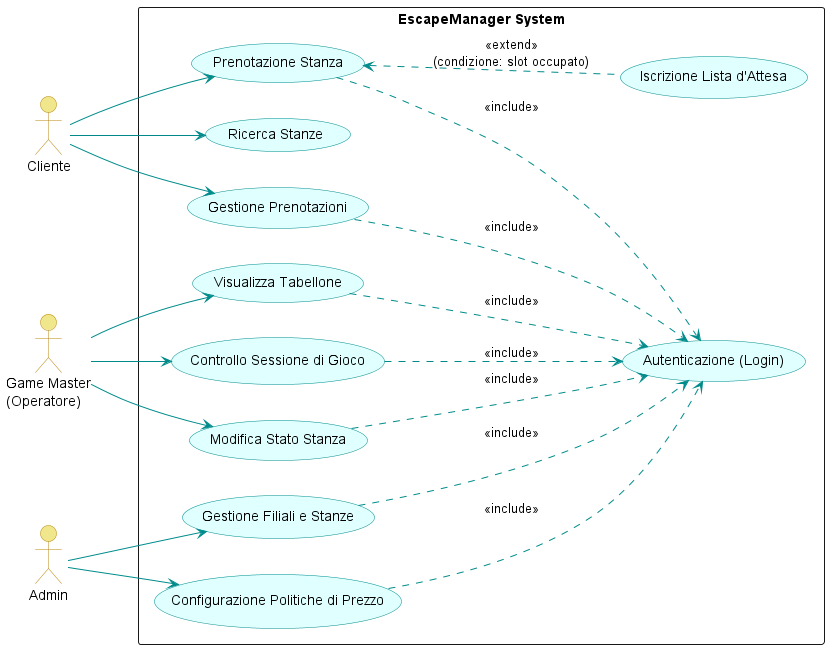
\includegraphics[width=0.85\textwidth]{images/usecase_diagram.png}
    \caption{Diagramma dei Casi d'Uso (Use Case Diagram) di EscapeManager}
    \label{fig:usecase}
\end{figure}

\section{Use Case Templates}
A corredo del diagramma, vengono definiti i template testuali per i casi d'uso primari. La formalizzazione di questi scenari descrive nel dettaglio il Flusso Base (Basic Flow) e i Flussi Alternativi (Alternative Flows), i quali costituiranno successivamente la base per la stesura dei test funzionali e di accettazione.

\subsection{UC1: Prenotazione Stanza}
Questo caso d'uso descrive il processo attraverso il quale un Cliente prenota una sessione di gioco in una specifica Escape Room, scegliendo data, ora e numero di partecipanti. Il sistema si occupa di verificare la disponibilità e calcolare la tariffa applicabile.

\begin{table}[H]
    \centering
    \renewcommand{\arraystretch}{1.3} % Aumenta lo spazio tra le righe
    \begin{tabularx}{\textwidth}{|l|X|}
        \hline
        \textbf{ID Caso d'Uso} & \textbf{UC1} \\
        \hline
        \textbf{Nome} & Prenotazione Stanza \\
        \hline
        \textbf{Attore Principale} & Cliente \\
        \hline
        \textbf{Pre-condizioni} & Il Cliente ha effettuato il login al sistema ed è autenticato. \\
        \hline
        \textbf{Post-condizioni} & Una nuova Prenotazione è registrata nel database, lo slot orario selezionato risulta occupato e il prezzo totale è stato calcolato e confermato. \\
        \hline
        \textbf{Flusso Base} & 
        \begin{minipage}[t]{\linewidth}
            \begin{enumerate}
                \item Il Cliente richiede di effettuare una nuova prenotazione.
                \item Il sistema mostra l'elenco delle filiali (Franchise) disponibili.
                \item Il Cliente seleziona una filiale.
                \item Il sistema mostra l'elenco delle Stanze associate alla filiale, indicando tema, difficoltà e capienza.
                \item Il Cliente seleziona una Stanza.
                \item Il sistema mostra il calendario con gli slot orari disponibili per i giorni futuri.
                \item Il Cliente seleziona una data, uno slot orario e inserisce il numero di giocatori previsti.
                \item Il sistema calcola il prezzo preventivato (applicando la \textit{PricingStrategy} attiva per quel giorno/stanza) e mostra il riepilogo.
                \item Il Cliente conferma la prenotazione.
                \item Il sistema registra la prenotazione, segna lo slot come non più disponibile e notifica al Cliente il successo dell'operazione.
            \end{enumerate}
        \end{minipage} \\
        \hline
        \textbf{Flussi Alternativi} & 
        \begin{minipage}[t]{\linewidth}
            \begin{itemize}
                \item \textbf{4a. Nessuna stanza disponibile:} Se la filiale non ha stanze attive, il sistema mostra un messaggio informativo e riporta il Cliente al passo 2.
                \item \textbf{7a. Violazione capienza:} Se il numero di giocatori inserito è inferiore al minimo o superiore alla capienza massima della stanza, il sistema mostra un messaggio di errore e richiede un nuovo inserimento (ritorno al passo 7).
                \item \textbf{9a. Slot occupato (Race Condition) / Estensione UC3:} Se nel lasso di tempo tra il passo 6 e il passo 9 un altro utente ha prenotato lo stesso slot, la conferma fallisce. Il sistema avvisa il Cliente e gli propone di iscriversi alla Lista d'Attesa (\textit{<<extend>> UC3}). Il flusso riprende dal passo 6.
            \end{itemize}
        \end{minipage} \\
        \hline
    \end{tabularx}
    \caption{Template descrittivo per UC1 - Prenotazione Stanza}
    \label{tab:uc1_prenotazione}
\end{table}
\chapter{Progettazione Architetturale e di Dominio}

Il processo di transizione dall'analisi dei requisiti alla progettazione ha seguito i principi dell'Object-Oriented Design (OOD) e l'approccio BCE (Boundary-Control-Entity). In questo capitolo viene dettagliata la struttura statica del Domain Model, ponendo particolare enfasi sull'applicazione dei Design Pattern fondamentali per garantire la manutenibilità, l'estensibilità e il disaccoppiamento del sistema.

\section{Architettura a Strati e BCE}
L'architettura è organizzata in strati coerenti con il paradigma BCE. Le interazioni tra Boundary (CLI e mockup), Control (Controllers) ed Entity (Domain Model) sono strettamente direzionali, mentre la persistenza è isolata nel layer DAO.

\begin{figure}[H]
    \centering
    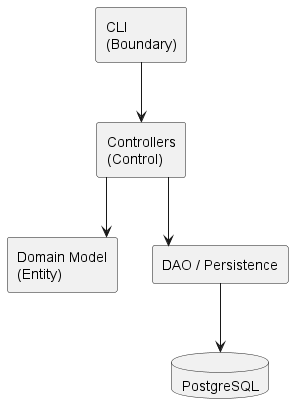
\includegraphics[width=\textwidth]{images/component_diagram.png}
    \caption{Architettura a strati e separazione BCE}
    \label{fig:component_diagram}
\end{figure}

\section{Package Diagram e Dipendenze}
Il Package Diagram (Figura \ref{fig:package_diagram}) descrive la struttura logica del progetto e le dipendenze tra i package principali. La CLI accede esclusivamente ai Controllers, i quali orchestrano Domain Model e DAO, mantenendo un flusso di dipendenze unidirezionale.

\begin{figure}[H]
    \centering
    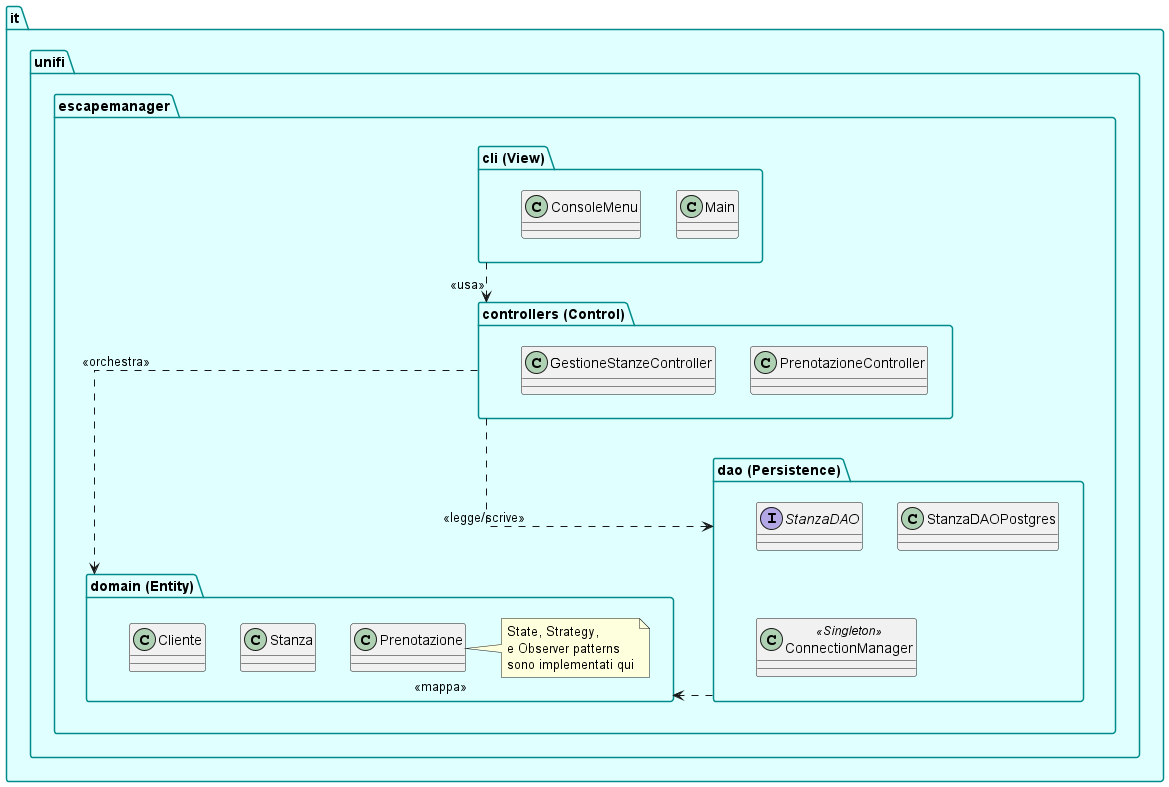
\includegraphics[width=0.75\textwidth]{images/package_diagram.png}
    \caption{Package Diagram dell'architettura di sistema}
    \label{fig:package_diagram}
\end{figure}

\section{Scelte Progettuali e Trade-off}
Ecco alcune scelte chiave adottate per mantenere il codice pulito e comprensibile:
\begin{itemize}
    \item \textbf{DAO + JDBC} invece di ORM: architettura leggera studiata per garantire maggiore controllo sul mapping e totale trasparenza dei flussi dati.
    \item \textbf{CLI come Boundary} per ridurre l'impatto della UI e concentrare lo sforzo sulla logica di business.
    \item \textbf{Pattern GoF espliciti} (State/Strategy/Observer) per rendere evidenti i punti di estensione del dominio.
    \item \textbf{Single Table Inheritance} per la gerarchia \texttt{Utente}, semplificando query e autenticazione futura.
\end{itemize}

\section{Domain Model (Class Diagram)}

La Figura \ref{fig:domain_model} illustra il diagramma delle classi per il nucleo dell'applicazione (Entity layer). Il modello non include volutamente i dettagli legati all'accesso ai dati (DAO) o all'interfaccia utente (View/CLI), concentrandosi esclusivamente sulle regole del franchise.

\begin{figure}[H]
    \centering
    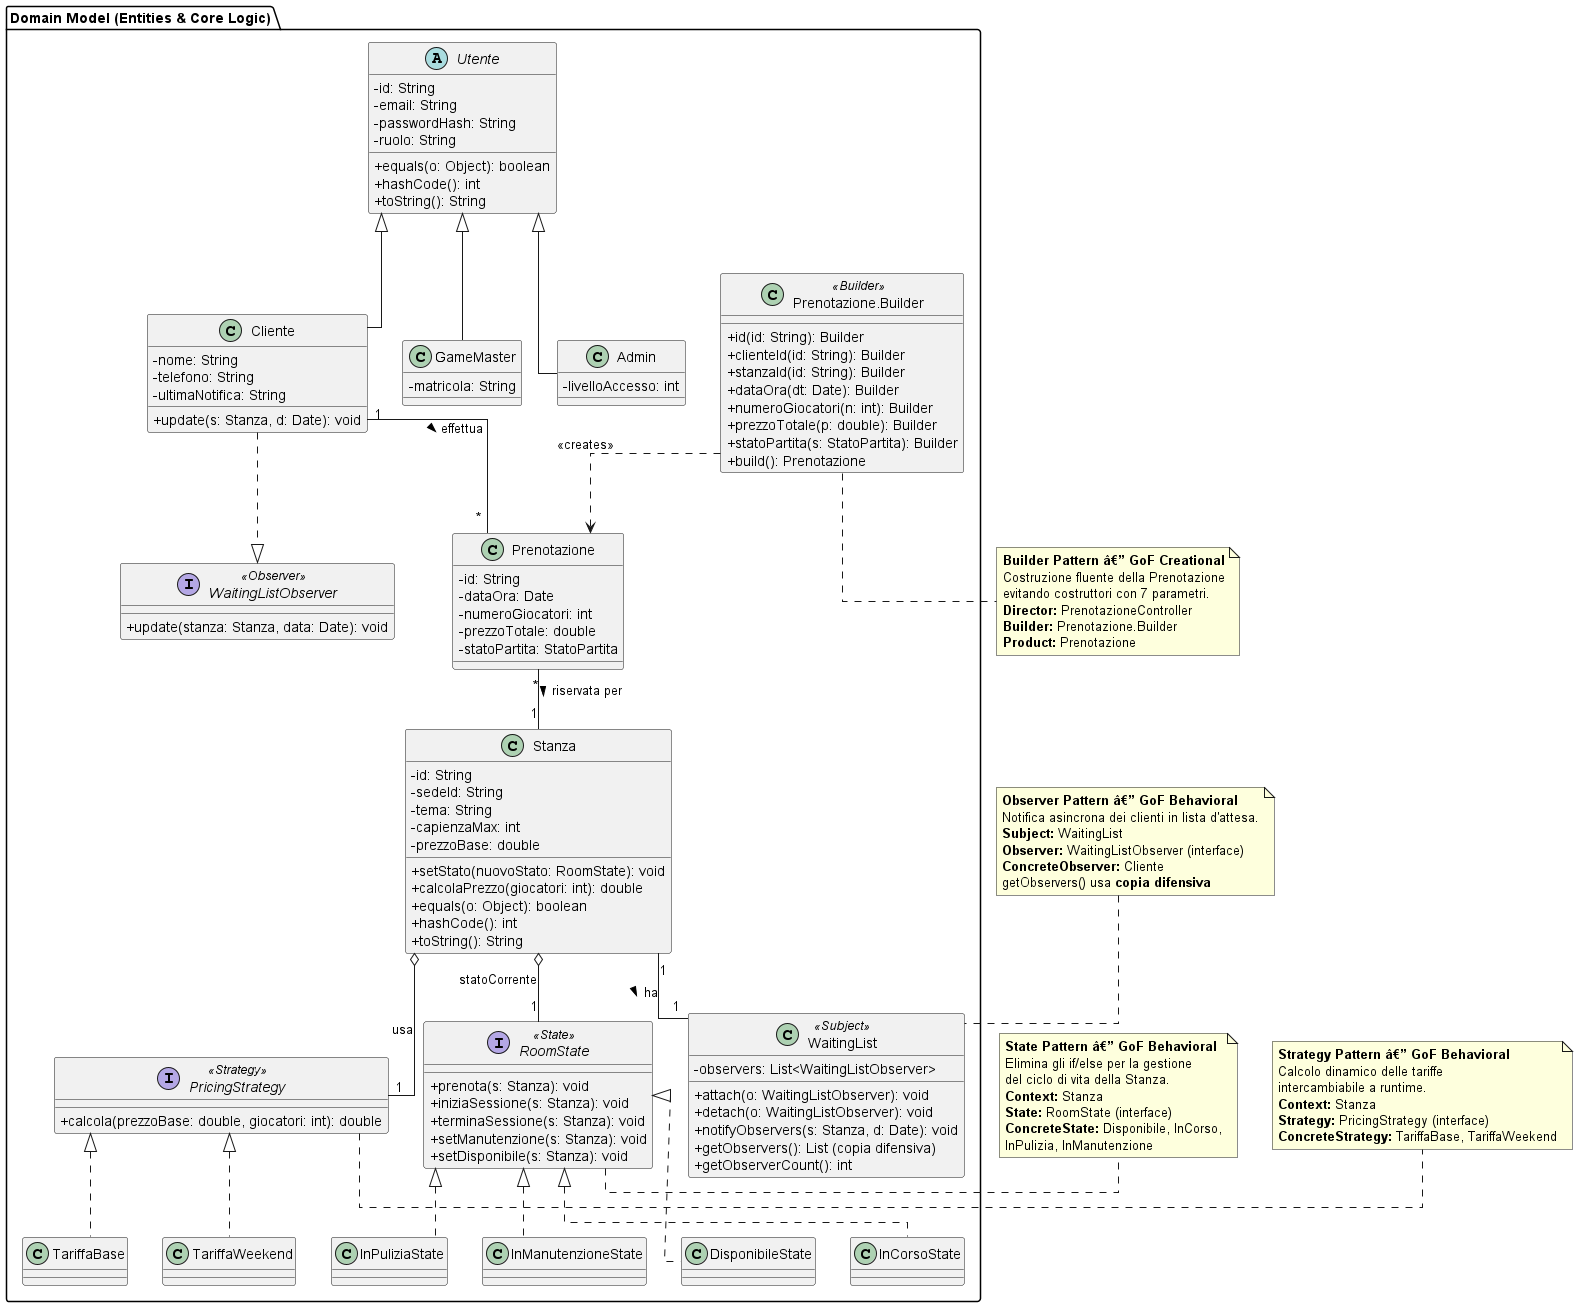
\includegraphics[width=1\textwidth]{images/domain_model.png}
    \caption{Diagramma delle Classi del Domain Model con Design Pattern}
    \label{fig:domain_model}
\end{figure}

\section{Class Diagram dei Controller e Boundary}
Per documentare i layer di controllo e presentazione, la Figura \ref{fig:class_diagram_controllers} mostra invece i Controllers (il livello Control) e la CLI (il livello Boundary).

\begin{figure}[H]
    \centering
    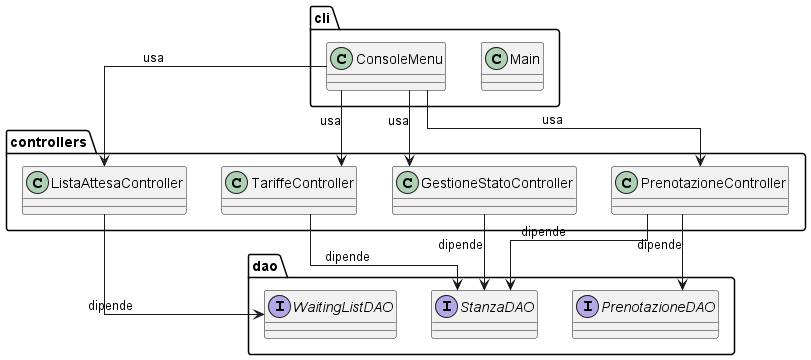
\includegraphics[width=0.9\textwidth]{images/class_diagram_controllers.png}
    \caption{Class Diagram: Controllers e Boundary (CLI)}
    \label{fig:class_diagram_controllers}
\end{figure}

\section{Class Diagram del Package DAO (Persistenza)}
Per non legare i Controller direttamente al database Postgres, il sistema usa il pattern \textbf{Abstract Factory} (DAO Factory). La Figura \ref{fig:class_diagram_dao} mostra il package \texttt{dao}, con le interfacce, le classi concrete e la connessione unica (Singleton).

\begin{figure}[H]
    \centering
    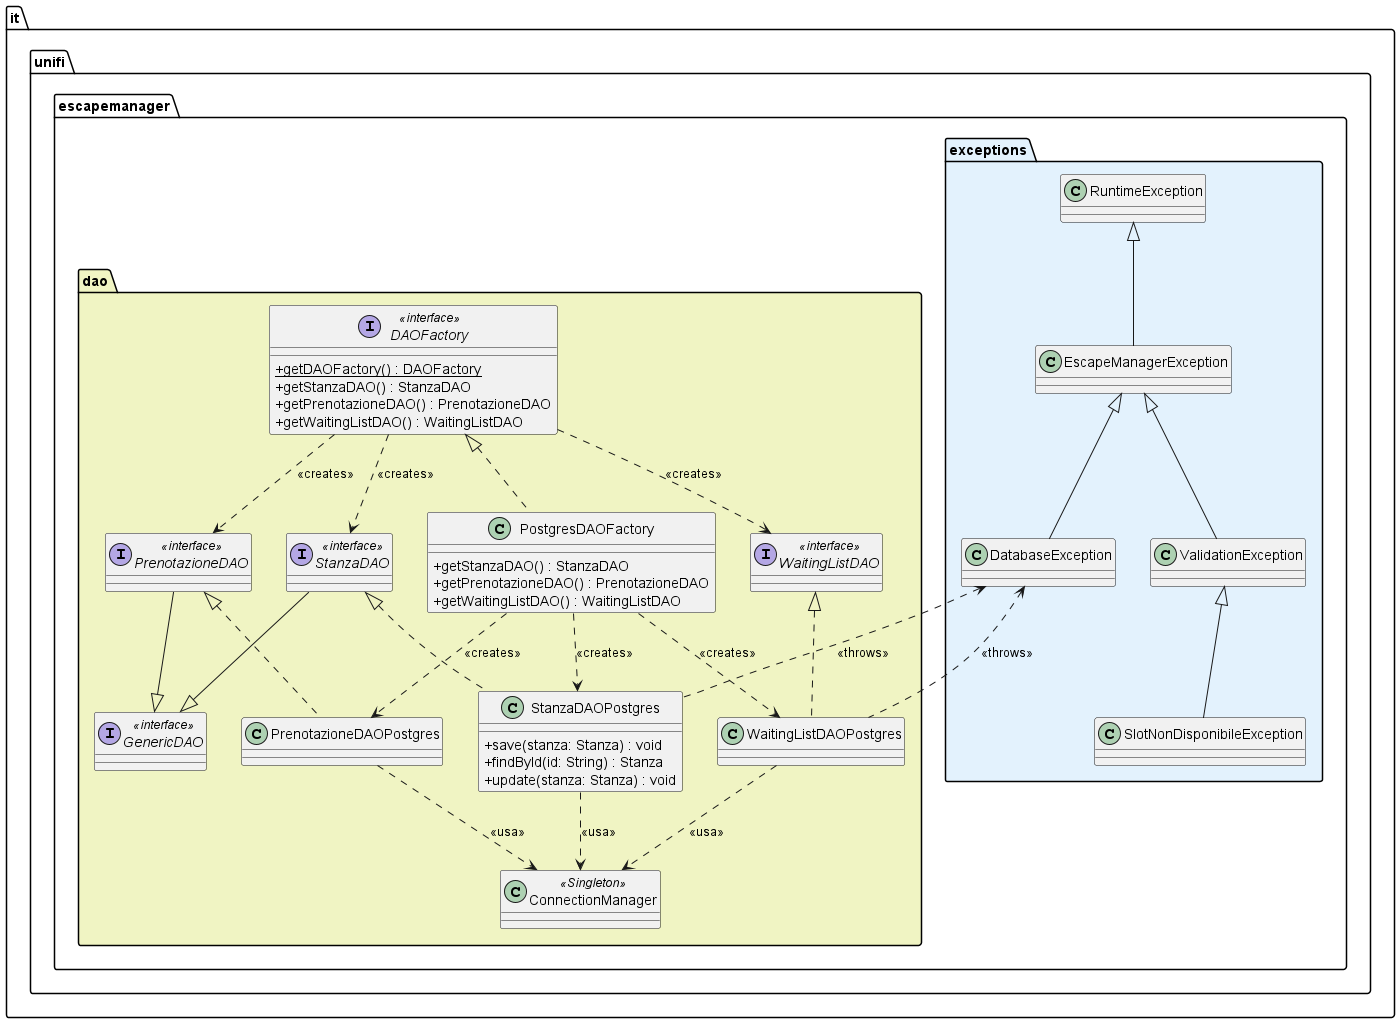
\includegraphics[width=0.95\textwidth]{images/class_diagram_persistence.png}
    \caption{Class Diagram: Package DAO e Gerarchia delle eccezioni}
    \label{fig:class_diagram_dao}
\end{figure}

\subsection{Scelte Architetturali e Design Pattern}

Per risolvere i problemi principali visti nei casi d'uso (Capitolo 2), ho inserito a livello di dominio tre Design Pattern della \textit{Gang of Four (GoF)}:

\begin{itemize}
    \item \textbf{State Pattern (Gestione ciclo di vita):} Come emerso nell'UC3, la \texttt{Stanza} attraversa fasi operative rigide (Disponibile, In Corso, In Pulizia, In Manutenzione). Invece di delegare il controllo a complessi blocchi \texttt{switch/case} basati su stringhe o enumerazioni, lo stato è stato reificato nell'interfaccia \texttt{RoomState}. Questo garantisce il rispetto del principio \textit{Open-Closed}: l'aggiunta di un nuovo stato futuro non richiederà la modifica del codice della classe \texttt{Stanza}.
    
    \item \textbf{Strategy Pattern (Politiche di Prezzo):} Le regole di tariffazione dipendono da fattori esterni (giorno della settimana, festività, tipologia di clienti). La classe \texttt{Stanza} delega il calcolo del costo totale all'interfaccia \texttt{PricingStrategy}. L'amministratore (UC4) può così iniettare a runtime strategie diverse (es. \texttt{TariffaBase} e \texttt{TariffaWeekend}) variando l'algoritmo di calcolo in modo trasparente.
    
    \item \textbf{Observer Pattern (Lista d'Attesa asincrona):} Per soddisfare il requisito dell'UC2 (Iscrizione Lista d'Attesa), è stato predisposto un meccanismo di Publish-Subscribe. La classe \texttt{WaitingList} agisce da \textit{Subject}, mantenendo una lista di \texttt{WaitingListObserver} (interfaccia implementata dal \texttt{Cliente}). L'infrastruttura di iscrizione è implementata e persiste su database; l'invio automatico delle notifiche è considerato un'estensione futura.
\end{itemize}

Oltre ai pattern, si sottolinea l'uso dell'ereditarietà per la gestione degli attori (\texttt{Utente} come classe astratta generalizzata) e la presenza di un riferimento a \texttt{Sede} tramite \texttt{sede\_id} nel modello dati, che consente di mantenere la coerenza con il concetto di franchising pur non essendo oggetto di operazioni dirette nella CLI.

\subsection{Object Diagram: Istanza Runtime del Pattern Observer}

Per illustrare concretamente il funzionamento del \textbf{Pattern Observer} (descritto nel Domain Model), la Figura \ref{fig:object_diagram} mostra un \textit{Object Diagram} rappresentativo di una specifica configurazione runtime del sistema.

\begin{figure}[H]
    \centering
    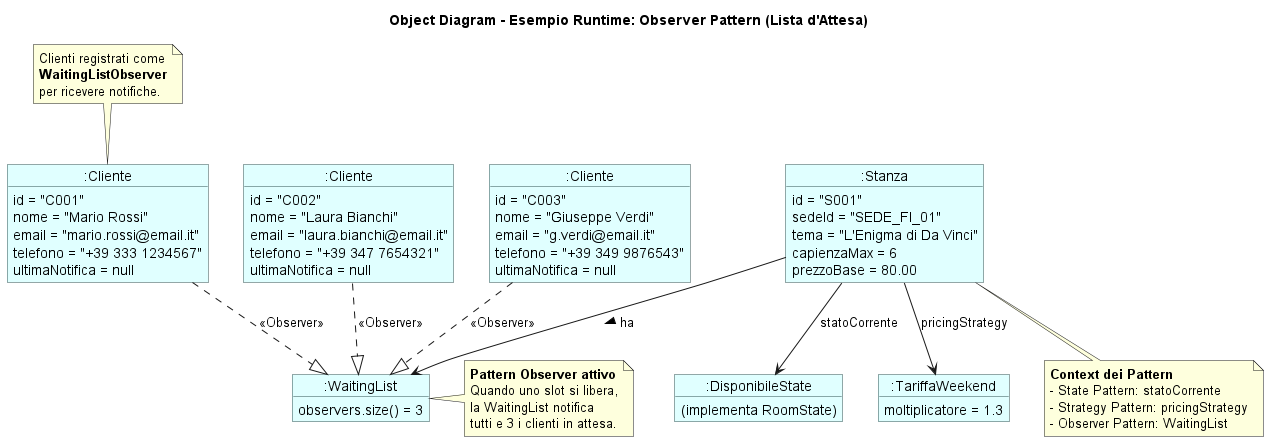
\includegraphics[width=0.95\textwidth]{images/object_diagram.png}
    \caption{Object Diagram: Esempio di istanza runtime del Pattern Observer (Lista d'Attesa)}
    \label{fig:object_diagram}
\end{figure}

L'Object Diagram raffigura tre clienti (\texttt{:Cliente}) registrati come osservatori (\texttt{WaitingList}\allowbreak\texttt{Observer}) sulla \texttt{:WaitingList} associata a una stanza specifica (\texttt{:Stanza}). Quando lo slot richiesto si libera, il Subject (\texttt{WaitingList}) invocherà il metodo \texttt{update()} su tutti e tre gli Observer, notificandoli della disponibilità.

Questo diagramma evidenzia inoltre le relazioni con i pattern \textbf{State} (stato corrente della stanza) e \textbf{Strategy} (politica di prezzo dinamica), mostrando come i tre pattern collaborino a runtime per realizzare la logica di business del franchising.

\subsection{State Machine Diagram}
Per documentare formalmente il ciclo di vita operativo della Stanza, è stato prodotto il diagramma a stati della Figura \ref{fig:state_machine_room}. Questo diagramma è una vista complementare al class diagram del Domain Model e descrive le transizioni valide tra i 4 stati concreti dell'interfaccia \texttt{RoomState}.

\begin{figure}[H]
    \centering
    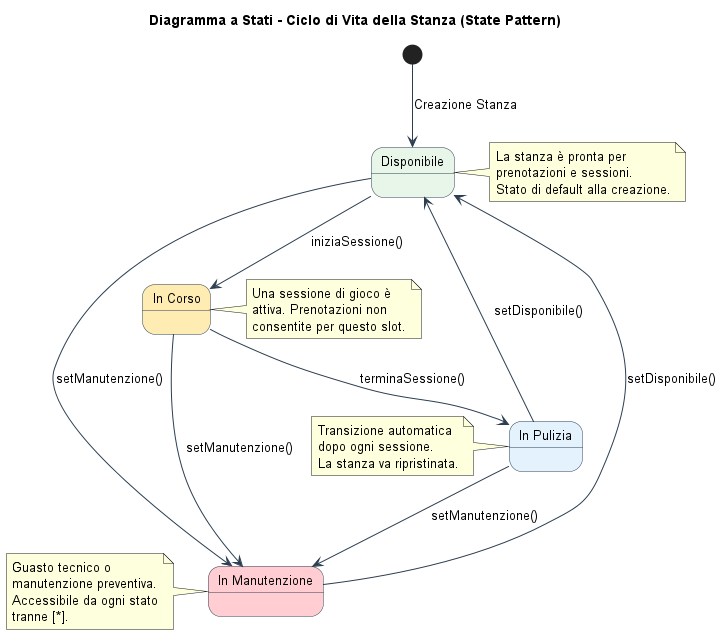
\includegraphics[width=0.85\textwidth]{images/state_machine_room.png}
    \caption{State Machine Diagram per il ciclo di vita della Stanza (RoomState)}
    \label{fig:state_machine_room}
\end{figure}


\section{Progettazione del Database}

Per salvare i dati, il Domain Model a oggetti è stato convertito in un database relazionale (PostgreSQL) usando specifiche strategie di mapping.

\subsection{Diagramma Entity-Relationship}

La Figura \ref{fig:er_diagram} mostra il diagramma Entità-Relazione (ER) del database, illustrando le tabelle principali, le chiavi primarie (PK) e i vincoli di chiave esterna (FK).

\begin{figure}[H]
    \centering
    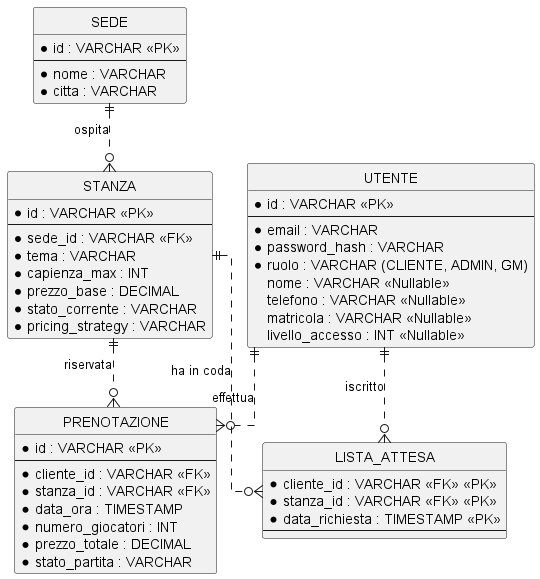
\includegraphics[width=0.85\textwidth]{images/er_diagram.png}
    \caption{Diagramma Entity-Relationship (ER) del sistema}
    \label{fig:er_diagram}
\end{figure}

\subsection{Strategie di Mapping e Modello Logico}

Per collegare il mondo a oggetti a quello delle tabelle ho scelto queste strade:

\begin{itemize}[leftmargin=*]
\raggedright
\setlength{\emergencystretch}{3em}
    \item \textbf{Mapping dell'Ereditarietà (Single Table Strategy):} La gerarchia della classe astratta \texttt{Utente} (Cliente, GameMaster, Admin) è stata mappata utilizzando il pattern \textit{Single Table Inheritance}. È stata creata un'unica tabella \texttt{UTENTE} provvista di una colonna discriminante (\texttt{ruolo}). Gli attributi specifici delle sottoclassi (es. \texttt{matricola} per il Game Master o \texttt{telefono} per il Cliente) sono stati resi \textit{nullable}. Questa scelta ottimizza le query di autenticazione evitando costose operazioni di \texttt{JOIN}.
    
    \item \textbf{Mapping dei Design Pattern (State e Strategy):} Le interfacce \texttt{RoomState} e \texttt{PricingStrategy} non diventano tabelle separate. Nella tabella \texttt{STANZA} sono persistite tramite stringhe (ad es.\ \texttt{stato\_corrente\allowbreak=\allowbreak IN\_MANUTENZIONE}). A livello di codice Java, i Data Access Object (DAO) utilizzano un meccanismo di \textit{Factory} per istanziare l'oggetto concreto corrispondente al valore letto dal database.
    
    \item \textbf{Associazioni Molti-a-Molti (Observer Pattern):} La logica Publish-Subscribe della Lista d'Attesa (UC2) si traduce relazionalmente nella tabella di \textit{junction} \texttt{LISTA\_ATTESA}. Questa tabella mappa la relazione N:N tra Clienti e Stanze, utilizzando una chiave primaria composita formata dalle foreign key e dal timestamp della richiesta.
\end{itemize}

\vspace{0.3cm}
\noindent Di seguito viene riportato lo \textbf{Schema Logico Relazionale} formalizzato:

\begin{itemize}[leftmargin=*]
\emergencystretch=3em
    \item \textbf{SEDE}(\underline{id}, nome, citta)
    \item \textbf{STANZA}(\underline{id}, \dashuline{sede\_id}, tema, capienza\_max, prezzo\_base, stato\_corrente, pricing\_strategy)
    \item \textbf{UTENTE}(\underline{id}, email, password\_hash, ruolo, nome*,\newline telefono*, matricola*, livello\_accesso*) --- {\small\textit{* attributo nullable a seconda del ruolo}}
    \item \textbf{PRENOTAZIONE}(\underline{id}, \dashuline{cliente\_id}, \dashuline{stanza\_id}, data\_ora, numero\_giocatori, prezzo\_totale, stato\_partita)
    \item \textbf{LISTA\_ATTESA}(\underline{\dashuline{cliente\_id}}, \underline{\dashuline{stanza\_id}}, \underline{data\_richiesta})
\end{itemize}

\section{Dinamica del Sistema (Implementation Perspective)}
Per illustrare le interazioni dinamiche tra gli oggetti a runtime, sono stati realizzati i Sequence Diagram per i casi d'uso principali.

\subsection{UC1 - Prenotazione Stanza}
La Figura \ref{fig:sequence_prenotazione} mostra il Sequence Diagram relativo al caso d'uso principale. Il diagramma evidenzia il rispetto del pattern architetturale BCE: l'interfaccia utente (Boundary) delega l'elaborazione al \texttt{PrenotazioneController} (Control), il quale orchestra il reperimento delle risorse persistenti e demanda la logica matematica di calcolo del prezzo all'entità \texttt{Stanza} (Entity). Particolare attenzione è stata posta nel disaccoppiamento del Controller dall'accesso ai dati, delegato interamente a un pattern creazionale.

\begin{figure}[H]
    \centering
    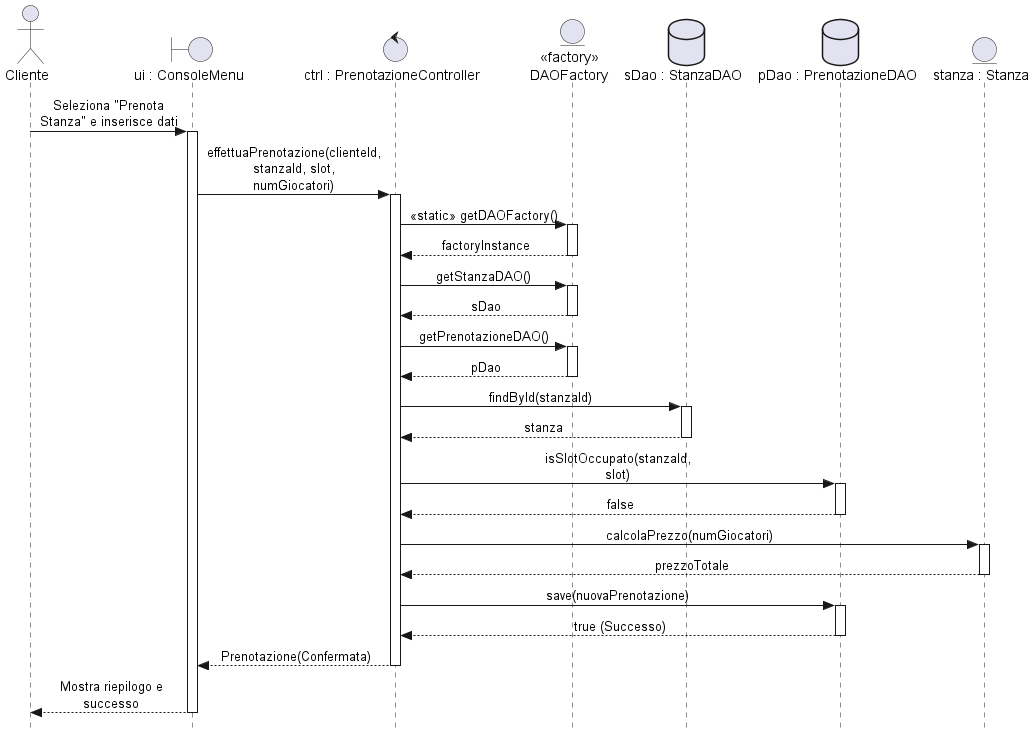
\includegraphics[width=\textwidth]{images/sequence_prenotazione.png}
    \caption{Sequence Diagram del caso d'uso UC1 (Prenotazione Stanza)}
    \label{fig:sequence_prenotazione}
\end{figure}

\subsection{UC4 - Configurazione Tariffe}
La Figura \ref{fig:sequence_tariffe} descrive il flusso di configurazione delle tariffe. L'Admin opera tramite la CLI, la quale delega al \texttt{TariffeController} la selezione della strategia e l'aggiornamento della stanza via DAO.

\begin{figure}[H]
    \centering
    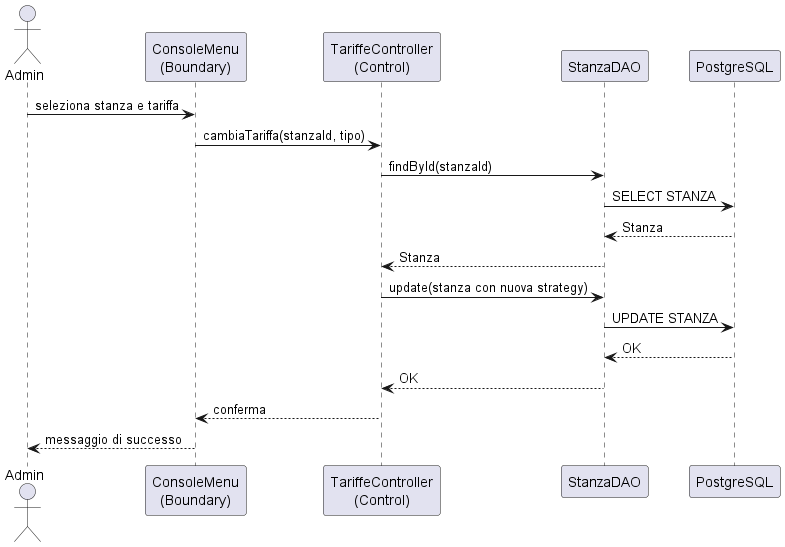
\includegraphics[width=0.95\textwidth]{images/sequence_tariffe.png}
    \caption{Sequence Diagram del caso d'uso UC4 (Configurazione Tariffe)}
    \label{fig:sequence_tariffe}
\end{figure}

\subsection{UC3 - Aggiornamento Stato Stanza}
La Figura \ref{fig:sequence_gestione_stato_cap3} mostra il Sequence Diagram per l'UC3, evidenziando la delega al \textbf{State Pattern}. Il Controller non contiene logica di stato: invoca il metodo di transizione sulla \texttt{Stanza}, la quale delega l'esecuzione all'oggetto \texttt{RoomState} corrente. Il diagramma include anche il flusso alternativo 4a (transizione non valida).

\begin{figure}[H]
    \centering
    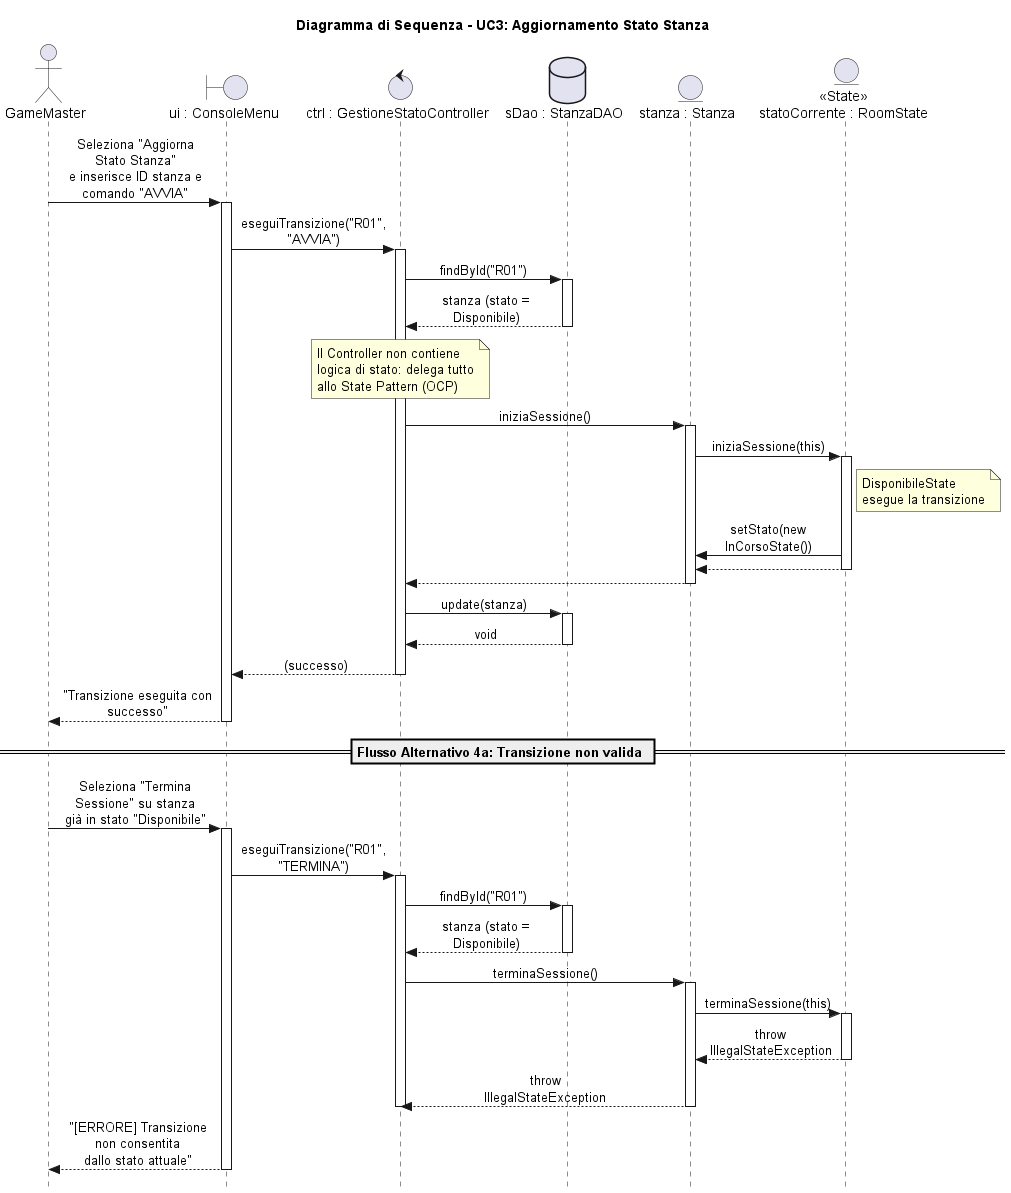
\includegraphics[width=0.95\textwidth]{images/sequence_gestione_stato.png}
    \caption{Sequence Diagram del caso d'uso UC3 (Aggiornamento Stato Stanza)}
    \label{fig:sequence_gestione_stato_cap3}
\end{figure}



\section{Pattern Creazionali: DAO Factory}
Nei diagrammi di sequenza si nota subito che, al momento di salvare i dati, ci si affida a una \textbf{DAO Factory} (Abstract Factory). 
L'idea è scollegare totalmente i Controller dal database PostgreSQL. Infatti, il Controller non crea mai una classe \texttt{StanzaDAOPostgres} usando \texttt{new}, ma si affida all'interfaccia esposta dalla Factory:

\begin{lstlisting}[language=Java, caption=Utilizzo del pattern DAO Factory nel Controller]
// Reperimento dinamico dei DAO indipendentemente dal DB sottostante
DAOFactory factory = DAOFactory.getDAOFactory();
StanzaDAO stanzaDao = factory.getStanzaDAO();
PrenotazioneDAO prenotazioneDao = factory.getPrenotazioneDAO();
\end{lstlisting}
Questo vuol dire che se un domani fosse necessario passare a MySQL, basterebbe creare una nuova Factory e i file SQL specifici, senza mai toccare il codice dei Controller o di Dominio.



\chapter{Implementazione e Architettura del Codice}

Questo capitolo mostra come il modello di dominio e lo schema del database sono stati trasformati in vero codice Java. Il progetto usa un'architettura "a strati" (Layered architecture) basata sul modello BCE, studiata per separare le responsabilità e semplificare la scrittura dei test.

\section{Architettura dei Package}

L'applicazione è organizzata in quattro package principali (Figura \ref{fig:package_diagram}). Le dipendenze tra i package sono rigorosamente direzionali: lo strato di presentazione (\texttt{cli}) non accede mai direttamente al database, ma passa per i \texttt{controllers}, che a loro volta orchestrano il \texttt{domain} e si interfacciano con i \texttt{dao}.

\subsection{cli (Boundary)}
Contiene il punto di ingresso dell'applicazione e la CLI. La classe \texttt{ConsoleMenu} gestisce l'interazione con l'utente, la validazione di input di base e la delega delle operazioni ai Controller.

\subsection{controllers (Control)}
Raccoglie i Controller che implementano i flussi dei casi d'uso. Ogni Controller incapsula la logica di coordinamento, chiama i DAO e applica le regole di business esposte dal Domain Model.

\subsection{domain (Entity)}
Include le entità di dominio (\texttt{Stanza}, \texttt{Prenotazione}, \texttt{Utente} e sottoclassi) e l'implementazione dei Design Pattern principali (State, Strategy, Observer).

\subsection{dao (Persistence)}
Contiene le interfacce DAO, le implementazioni PostgreSQL e l'oggetto \texttt{ConnectionManager}. L'obiettivo è isolare la persistenza e mantenere il dominio indipendente dalla tecnologia di storage.

\section{Livello di Persistenza (Pattern DAO)}

Per non mischiare la logica dell'applicazione con il codice SQL, l'accesso a PostgreSQL è gestito dal pattern \textbf{Data Access Object (DAO)}. In questo modo la business logic non sa (e non deve sapere) nulla di come funziona materialmente il database.

La connessione al database è gestita tramite un \textbf{Singleton Pattern} (\texttt{ConnectionManager}), che assicura l'esistenza di un'unica istanza di connessione (o di un connection pool) condivisa per tutta l'applicazione, evitando l'overhead di connessioni multiple.

\begin{lstlisting}[caption={Interfaccia generica DAO (\texttt{GenericDAO.java})}, label={lst:dao_interface}]
public interface GenericDAO<T, ID> {
    void save(T entity);
    T findById(ID id);
    List<T> findAll();
    void update(T entity);
    void delete(ID id);
}
\end{lstlisting}

\begin{lstlisting}[caption={Specializzazione per il dominio (\texttt{StanzaDAO.java})}, label={lst:stanza_dao}]
public interface StanzaDAO extends GenericDAO<Stanza, String> {
    List<Stanza> findBySedeAndStato(String sedeId, String statoCorrente);
}
\end{lstlisting}

In modo analogo, \texttt{PrenotazioneDAO} e \texttt{WaitingListDAO} incapsulano le operazioni di persistenza per prenotazioni e liste d'attesa.

\section{Configurazione della Connessione al Database}
Le credenziali di accesso al database non sono hardcoded: vengono lette da \texttt{db.properties} (in \texttt{src/main/resources}) o da variabili d'ambiente, separando configurazione e codice ed evitando la pubblicazione accidentale di segreti.

\begin{lstlisting}[caption={Caricamento della configurazione DB dal classpath}]
Properties props = loadProperties();
String url = firstNonBlank(
    System.getenv("EM_DB_URL"),
    System.getProperty("db.url"),
    props.getProperty("db.url"),
    "jdbc:postgresql://localhost:5432/escapemanager"
);
\end{lstlisting}

\section{Validazione Input e Gestione Errori}
La CLI valida i formati di input (numeri, date e orari) prima di invocare i Controller. Le eccezioni di business (\texttt{ValidationException} e sottoclassi) propagano errori gestibili dalla UI, mantenendo la logica di validazione separata dalla presentazione.

\section{Implementazione dei Design Pattern}

Di seguito vengono riportati i frammenti di codice più significativi che mostrano l'implementazione pratica dei Design Pattern progettati nel Capitolo 3.

\subsection{State Pattern}
Lo State Pattern elimina la necessità di costrutti condizionali complessi per la gestione del ciclo di vita della \texttt{Stanza}. Ogni stato concreto implementa il comportamento specifico e gestisce, ove necessario, la transizione allo stato successivo.

\begin{lstlisting}[caption={Interfaccia dello State Pattern (\texttt{RoomState.java})}, label={lst:state_interface}]
public interface RoomState {
    void prenota(Stanza stanza);
    void iniziaSessione(Stanza stanza);
    void terminaSessione(Stanza stanza);
    void setManutenzione(Stanza stanza);
    void setDisponibile(Stanza stanza);
    String getStatusString();
}
\end{lstlisting}

\begin{lstlisting}[caption={Stato concreto (\texttt{DisponibileState.java})}, label={lst:state_concrete}]
public class DisponibileState implements RoomState {
    @Override
    public void iniziaSessione(Stanza stanza) {
        stanza.setStato(new InCorsoState()); // Transizione di stato
    }
    
    @Override
    public void terminaSessione(Stanza stanza) {
        throw new IllegalStateException(
            "Impossibile terminare una sessione per una stanza DISPONIBILE.");
    }
    // ... altri metodi
}
\end{lstlisting}

\begin{approfondimento}
\textbf{State Pattern vs Strategy Pattern}

Lo \textbf{State Pattern} e lo \textbf{Strategy Pattern} condividono la stessa struttura meccanica: entrambi delegano il comportamento a un oggetto che implementa un'interfaccia comune, favorendo il polimorfismo rispetto ai costrutti condizionali. Tuttavia, differiscono nell'\textit{intento}:
\begin{itemize}
    \item \textbf{Strategy}: l'algoritmo viene scelto \textit{una tantum} dall'esterno (es. l'Admin seleziona \texttt{TariffaWeekend}) e resta fisso per la durata dell'operazione. Le strategie sono intercambiabili ma non si sostituiscono autonomamente.
    \item \textbf{State}: l'oggetto \textit{transiziona automaticamente} tra stati in base alla propria logica interna. Ad esempio, \texttt{DisponibileState} sa che dopo \texttt{iniziaSessione()} lo stato diventa \texttt{InCorsoState}. La transizione è governata dallo stato stesso, non dal client.
\end{itemize}
Nel progetto, questa distinzione è evidente: la \texttt{PricingStrategy} viene impostata esplicitamente dal \texttt{TariffeController}. Al contrario, il \texttt{RoomState} si auto-sostituisce: ogni stato concreto invoca \texttt{stanza.setStato()} all'interno dei propri metodi di transizione, senza intervento esterno.
\end{approfondimento}

\subsection{Strategy Pattern}
Il calcolo del prezzo della prenotazione (UC1) è demandato alla \texttt{PricingStrategy}. L'Admin, tramite il \texttt{TariffeController}, seleziona la strategia appropriata e la imposta sulla stanza.

\begin{lstlisting}[caption={Interfaccia dello Strategy Pattern (\texttt{PricingStrategy.java})}, label={lst:strategy_interface}]
public interface PricingStrategy {
    double calcola(double prezzoBase, int numeroGiocatori);
}
\end{lstlisting}

\begin{lstlisting}[caption={Strategia concreta (\texttt{TariffaWeekend.java})}, label={lst:strategy_concrete}]
public class TariffaWeekend implements PricingStrategy {
    private static final double SOVRAPPREZZO = 1.20; // +20%
    
    @Override
    public double calcola(double prezzoBase, int numeroGiocatori) {
        return (prezzoBase * numeroGiocatori) * SOVRAPPREZZO;
    }
}
\end{lstlisting}

\subsection{Observer Pattern}
La lista d'attesa (UC2) implementa un sistema Publisher-Subscriber puro in Java, disaccoppiando l'evento di cancellazione di una prenotazione dall'invio effettivo delle notifiche.

\begin{lstlisting}[caption={Interfaccia Observer (\texttt{WaitingListObserver.java})}, label={lst:observer_interface}]
public interface WaitingListObserver {
    void update(Stanza stanza, LocalDateTime slotLiberato);
}
\end{lstlisting}

\begin{lstlisting}[caption={Subject concreto (\texttt{WaitingList.java})}, label={lst:observer_subject}]
public class WaitingList {
    private List<WaitingListObserver> observers = new ArrayList<>();

    public void attach(WaitingListObserver observer) {
        observers.add(observer);
    }

    public void notifyObservers(Stanza stanza, LocalDateTime slot) {
        for (WaitingListObserver obs : observers) {
            obs.update(stanza, slot);
        }
    }
}
\end{lstlisting}

\subsection{Builder Pattern}
La classe \texttt{Prenotazione} richiede 7 parametri diversi nel costruttore. Per evitare confusione con l'ordine delle variabili ho usato il pattern creazionale \textbf{Builder}, che rende il codice molto più leggibile quando si devono inizializzare molti attributi.

\begin{lstlisting}[caption={Builder Pattern per la classe Prenotazione}, label={lst:builder_pattern}]
Prenotazione p = new Prenotazione.Builder()
        .id(UUID.randomUUID().toString())
        .clienteId("C01")
        .stanzaId("R01")
        .dataOra(LocalDateTime.of(2026, 10, 31, 21, 0))
        .numeroGiocatori(4)
        .prezzoTotale(80.0)
        .statoPartita("CONFERMATA")
        .build();
\end{lstlisting}

\section{Dependency Injection e Testabilità}
I Controller ricevono i DAO tramite costruttore, facilitando la sostituzione delle dipendenze in fase di test. La CLI si limita a comporre l'oggetto e a delegare, mantenendo separati input/output e logica di business.

\begin{lstlisting}[language=Java, caption=Iniezione delle dipendenze nel controller]
PrenotazioneDAO prenotazioneDAO = factory.getPrenotazioneDAO();
StanzaDAO stanzaDAO = factory.getStanzaDAO();
PrenotazioneController controller = new PrenotazioneController(prenotazioneDAO, stanzaDAO);
\end{lstlisting}

\section{Gestione Centralizzata delle Eccezioni (Information Hiding)}
Per il controllo degli errori ho evitato le eccezioni base di Java (come \texttt{RuntimeException}), preferendo una gerarchia di eccezioni custom derivata da \texttt{EscapeManagerException}.

Come illustrato nella Figura \ref{fig:class_diagram_persistence}, la gerarchia divide formalmente gli errori in base al layer architetturale in cui si verificano:
\begin{itemize}
    \item \textbf{\texttt{ValidationException}:} utilizzata dal dominio per segnalare violazioni delle invarianti di business (es. la sottoclasse \texttt{SlotNonDisponibileException}).
    \item \textbf{\texttt{DatabaseException}:} utilizzata dal layer DAO per incapsulare problemi di persistenza.
\end{itemize}

\begin{figure}[H]
    \centering
    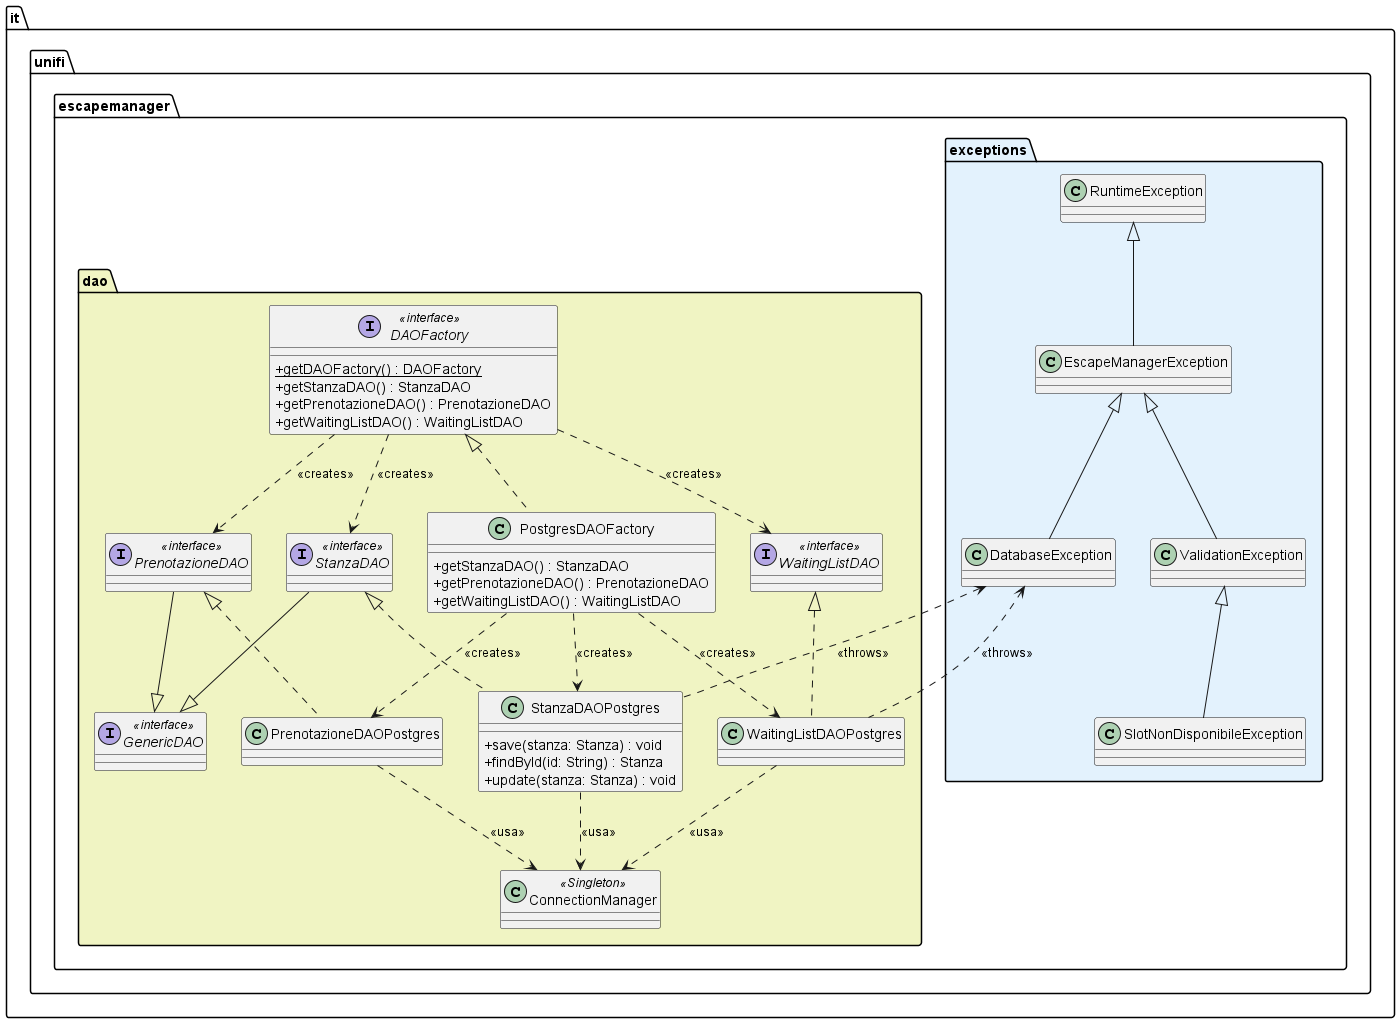
\includegraphics[width=0.85\textwidth]{images/class_diagram_persistence.png}
    \caption{Diagramma delle Classi: Pattern DAO Factory e Gerarchia Eccezioni}
    \label{fig:class_diagram_persistence}
\end{figure}

Questo approccio maschera i dettagli tecnici (Information Hiding): se il driver JDBC lancia una \texttt{SQLException}, il livello DAO la cattura e la trasforma in una \texttt{DatabaseException}. Così facendo, il Controller che riceve l'errore non deve preoccuparsi di questioni legate a SQL o al driver.

\begin{lstlisting}[language=Java, caption=Incapsulamento delle eccezioni SQL nel layer DAO]
try (PreparedStatement stmt = conn.prepareStatement(query)) {
    // Esecuzione query...
} catch (SQLException e) {
    // La SQLException originaria viene nascosta ai livelli superiori
    throw new DatabaseException("Errore di accesso ai dati durante il salvataggio.", e);
}
\end{lstlisting}

\section{Gerarchia delle Interfacce e Liskov Substitution Principle}
Ho creato l'interfaccia \texttt{GenericDAO<T, ID>} per avere un contratto di base CRUD per tutte le entità. Le sotto-interfacce come \texttt{StanzaDAO} aggiungono le interrogazioni specifiche, e le classi concrete come \texttt{StanzaDAOPostgres} contengono le vere query SQL. 

Questo design rispetta il \textbf{Liskov Substitution Principle (LSP)}: il blocco dei \textit{Controller} comunica solo con l'astrazione (\texttt{StanzaDAO}) e ignora totalmente quale sia la classe concreta fornita in quel momento.

\begin{lstlisting}[language=Java, caption=Gerarchia delle interfacce DAO]
public interface GenericDAO<T, ID> {
    void save(T entity);
    T findById(ID id);
    List<T> findAll();
    void update(T entity);
    void delete(ID id);
}

// Specializzazione per il dominio: aggiunge query domain-specific
public interface StanzaDAO extends GenericDAO<Stanza, String> {
    List<Stanza> findBySedeAndStato(String sedeId, String statoCorrente);
}
\end{lstlisting}

\section{Copia Difensiva (Defensive Copy)}
Per tenere al sicuro i dati ho usato una tecnica chiamata \textbf{copia difensiva}. La classe \texttt{WaitingList} contiene internamente la lista degli iscritti (Observer). Se fornissi la lista tramite un classico getter, chiunque potrebbe manipolarla dall'esterno. Per proteggerla (Information Hiding), \texttt{getObservers()} ne restituisce una versione in sola lettura:

\begin{lstlisting}[language=Java, caption=Copia difensiva nella WaitingList]
public List<WaitingListObserver> getObservers() {
    return Collections.unmodifiableList(observers);
}
\end{lstlisting}

Qualsiasi tentativo di aggiungere o rimuovere elementi dalla lista restituita causerà una \texttt{UnsupportedOperationException}, proteggendo l'integrità dell'incapsulamento.




\chapter{Collaudo e Testing}

La fase di verifica e validazione del sistema \textbf{EscapeManager} è stata condotta seguendo un approccio multilivello, utilizzando il framework \textbf{JUnit 5}. L'obiettivo del collaudo non è stato solo quello di garantire l'assenza di difetti evidenti (bug), ma soprattutto di dimostrare la robustezza dell'architettura e la perfetta aderenza ai requisiti funzionali delineati nel Capitolo 2.

\section{Strategia di Verifica}
La strategia di test è organizzata su tre livelli:
\begin{itemize}
    \item \textbf{Unit Test (White-Box):} verificano le logiche pure del Domain Model e dei Design Pattern.
    \item \textbf{Integration Test (DAO/DB):} verificano il mapping ORM e la correttezza delle query principali.
    \item \textbf{Functional Test (Black-Box):} esercitano i Controller come surrogati della UI, in linea con i template UC.
\end{itemize}

\section{Setup e Dati di Test}
Per garantire test ripetibili, prima di ogni test di integrazione o funzionale il database viene riportato ad uno stato noto tramite \texttt{DatabaseHelper.resetTestDatabase()}, che esegue TRUNCATE e reinserisce dati minimi consistenti (una stanza e due clienti).

\section{Testing Strutturale (White-Box)}

I test strutturali (o Unit Test) si sono concentrati sulle classi del \texttt{Domain Model}, con l'obiettivo di massimizzare la copertura (Code Coverage) dei rami condizionali e verificare la correttezza algoritmica, in totale isolamento dalle dipendenze esterne.

Particolare attenzione è stata dedicata al collaudo dei Design Pattern. Il Listing \ref{lst:test_strategy} mostra un test parametrizzato per la verifica delle politiche di prezzo dinamiche (\textit{Strategy Pattern}).

\begin{lstlisting}[caption={Unit Test per la logica di calcolo del prezzo (Strategy Pattern)}, label={lst:test_strategy}]
class PricingStrategyTest {

    @Test
    void testTariffaBaseCalcoloCorretto() {
        // Setup
        Stanza stanza = new Stanza("R01", "FI01", "Horror Asylum", 6, 20.0);
        stanza.setPricingStrategy(new TariffaBase());
        
        // Execution: 4 giocatori a 20 euro base = 80 euro
        double prezzoCalcolato = stanza.calcolaPrezzo(4);
        
        // Assertion
        assertEquals(80.0, prezzoCalcolato);
    }
}
\end{lstlisting}

Oltre al calcolo del prezzo, i test unitari verificano anche le transizioni di stato della \texttt{Stanza} (State Pattern) e la corretta gestione delle eccezioni in caso di transizioni non valide.

\section{Testing di Integrazione (DAO e Database)}

Per verificare il corretto interfacciamento tra l'applicazione Java e il database PostgreSQL (livello ORM), sono stati implementati test di integrazione sulle classi DAO.
Per garantire la \textbf{ripetibilità} e l'isolamento, il costrutto \texttt{@BeforeEach} invoca \texttt{DatabaseHelper.resetTestDatabase()}, che esegue TRUNCATE e reinserisce un dataset minimo prima di ogni metodo di test.

\begin{lstlisting}[caption={Integration Test per StanzaDAOPostgres con reset dello stato}, label={lst:test_dao}]
class StanzaDAOPostgresTest {
    private StanzaDAO stanzaDao;

    @BeforeEach
    void setUp() {
        DatabaseHelper.resetTestDatabase();
        stanzaDao = DAOFactory.getDAOFactory().getStanzaDAO();
    }

    @Test
    void testSaveAndFindById() {
        Stanza stanza = stanzaDao.findById("R01");
        assertNotNull(stanza);
        assertEquals("Horror Asylum", stanza.getTema());
    }
}
\end{lstlisting}

\section{Testing Funzionale (Black-Box e Tracciabilità)}

Il livello più alto di collaudo ha riguardato i \texttt{Controllers}. In questa fase (Black-Box Testing) la logica interna viene ignorata e il sistema viene testato esclusivamente in base agli input e agli output attesi.

Per garantire la massima \textbf{tracciabilità}, ogni test funzionale è stato mappato direttamente su uno specifico \textit{Use Case Template} (Sezione 2.2). Sono stati collaudati sia i \textit{Flussi Base} che i \textit{Flussi Alternativi} (le eccezioni).

Il Listing \ref{lst:test_funzionale} dimostra come il sistema gestisce fluidamente la \textit{Race Condition} descritta nell'UC1 (Alternativa 3a), negando la prenotazione se lo slot risulta già occupato a database.

\begin{lstlisting}[caption={Functional Test tracciato sull'UC1 (Flusso Alternativo 3a)}, label={lst:test_funzionale}]
class PrenotazioneControllerTest {
    private PrenotazioneController controller;
    private PrenotazioneDAO prenotazioneDAO;

    @BeforeEach
    void setUp() {
        DatabaseHelper.resetTestDatabase();
        DAOFactory factory = DAOFactory.getDAOFactory();
        prenotazioneDAO = factory.getPrenotazioneDAO();
        StanzaDAO stanzaDAO = factory.getStanzaDAO();
        controller = new PrenotazioneController(prenotazioneDAO, stanzaDAO);
    }

    @Test
    void testPrenotazioneNegataPerSlotOccupato_UC1_Alt3a() {
        // Setup: Il Cliente 2 tenta di prenotare uno slot appena occupato dal Cliente 1
        String stanzaId = "R01";
        LocalDateTime slotRichiesto = LocalDateTime.of(2026, 10, 31, 21, 0);
        
        // Simulo la race condition pre-occupando lo slot via DAO
        Prenotazione esistente = new Prenotazione(
            UUID.randomUUID().toString(), "CLIENTE_01", stanzaId,
            slotRichiesto, 3, 60.0, "CONFERMATA");
        prenotazioneDAO.save(esistente);

        // Execution & Assertion
        SlotNonDisponibileException eccezione = assertThrows(
            SlotNonDisponibileException.class, 
            () -> controller.effettuaPrenotazione("CLIENTE_02", stanzaId, slotRichiesto, 4)
        );
        
        assertEquals("Lo slot orario selezionato non e' piu' disponibile.", eccezione.getMessage());
    }
}
\end{lstlisting}

\subsection{Catalogo dei Test}
La Tabella \ref{tab:test_catalog} riassume l'intera suite di test, indicando tipo e identificativo.

\begin{table}[H]
    \centering
    \small
    \renewcommand{\arraystretch}{1.2}
    \begin{tabularx}{\textwidth}{|>{\bfseries}l|>{\bfseries}l|X|}
        \hline
        ID & Tipo & Test \\ \hline
        U1 & Unit & \texttt{PricingStrategyTest.testTariffaBaseCalcoloCorretto} \\ \hline
        U2 & Unit & \texttt{StanzaTest.testTransizioneCorretta} \\ \hline
        U3 & Unit & \texttt{StanzaTest.testEccezioneStatoNonValido} \\ \hline
        I1 & Integration & \texttt{StanzaDAOPostgresTest.testSaveAndFindById} \\ \hline
        F1 & Functional & \texttt{PrenotazioneControllerTest.testPrenotazioneNegataPerSlotOccupato\_UC1\_Alt3a} \\ \hline
        F2 & Functional & \texttt{ListaAttesaControllerTest.testIscrizioneListaAttesa\_OK} \\ \hline
        F3 & Functional & \texttt{ListaAttesaControllerTest.testIscrizioneListaAttesa\_Duplicato} \\ \hline
        F4 & Functional & \texttt{GestioneStatoControllerTest.testEseguiTransizioneAvvia} \\ \hline
        F5 & Functional & \texttt{GestioneStatoControllerTest.testTransizioneNonValida\_TerminaSuDisponibile\_UC3\_Alt4a} \\ \hline
        F6 & Functional & \texttt{TariffeControllerTest.testCambioTariffaWeekend\_UC4} \\ \hline
    \end{tabularx}
    \caption{Catalogo dei test (unit, integrazione, funzionali)}
    \label{tab:test_catalog}
\end{table}

\subsection{Tracciabilità Use Case \textrightarrow{} Test}
I test funzionali F1--F6 sono tracciati direttamente sui template del Capitolo 2. La Tabella \ref{tab:traceability} sintetizza la copertura dei flussi base e alternativi.

\begin{table}[H]
    \centering
    \small
    \renewcommand{\arraystretch}{1.2}
    \begin{tabularx}{\textwidth}{|>{\bfseries}l|X|}
        \hline
        Use Case / Flusso & Test ID \\ \hline
        UC1 - Flusso alternativo 3a (slot occupato) & F1 \\ \hline
        UC2 - Flusso base (iscrizione) & F2 \\ \hline
        UC2 - Alternativa 5a (duplicato) & F3 \\ \hline
        UC3 - Flusso base (avvio sessione) & F4 \\ \hline
        UC3 - Alternativa 4a (transizione non valida) & F5 \\ \hline
        UC4 - Flusso base (cambio tariffa) & F6 \\ \hline
    \end{tabularx}
    \caption{Matrice di tracciabilità Use Case \textrightarrow{} Test}
    \label{tab:traceability}
\end{table}

\section{Risultati}
La suite di test è composta da \textbf{7 classi} e \textbf{10 test cases}, distribuiti tra unit, integrazione e test funzionali. Non è stata eseguita una misura formale di coverage, ma i test coprono i principali rami decisionali dei pattern e i flussi alternativi più critici nei casi d'uso.

\section{Conclusioni}

L'approccio metodologico adottato, guidato dai principi dell'Object-Oriented Design e supportato dall'uso estensivo dei Design Pattern, ha permesso di sviluppare \textbf{EscapeManager} come un sistema robusto, altamente coeso e disaccoppiato. 
La suite di collaudo ha confermato la solidità della logica di business e la corretta integrazione con il layer relazionale, soddisfacendo integralmente i requisiti posti in fase di analisi e fornendo un'architettura facilmente estensibile per sviluppi futuri (es. integrazione di sensori fisici nelle stanze tramite \textit{Adapter Pattern} o implementazione di un'interfaccia grafica avanzata al posto dell'attuale CLI).




\end{document}